\documentclass{article}
\usepackage{fullpage}
\usepackage[czech]{babel}
\usepackage{amsfonts}
\usepackage{graphicx}
\usepackage{caption}
\graphicspath{{images/}}

\title{\vspace{-2cm}Fyzika 24. 2. 2023\vspace{-1.7cm}}
\date{}
\author{}

\begin{document}
\maketitle

\section{Deformace}

  \begin{minipage}{0.25\textwidth}\raggedleft
    \begin{itemize}
      \item typy:
      \begin{itemize}
        \item tahem/tlakem
        \item kroucením
        \item ohybem
        \item smykem
      \end{itemize}
    \end{itemize}
  \end{minipage}
  \hspace{0.5cm}
  \noindent\begin{minipage}{0.12\textwidth}
    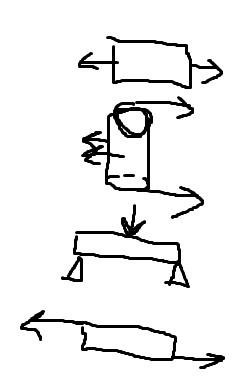
\includegraphics[width=0.9\linewidth]{deformace}
  \end{minipage}

  \subsection{Deformace tahem/tlakem}

    \begin{itemize}
      \item Normálové nápětí:
      	\begin{equation}
          \sigma=F/S; \ [N/m^2] = [Pa]
        \end{equation}
        \begin{center}
          \vspace{-0.25cm}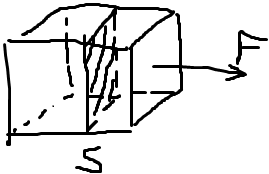
\includegraphics[width=0.12\textwidth]{normalove_napeti}\vspace{-0.25cm}
        \end{center}
      \item Změna délky:
        \begin{equation}
          \Delta l = l - l_0; \ [m]
        \end{equation}
      užitečnější většinou relativní prodloužení:
        \begin{equation}
          \varepsilon = \Delta l/l_0; \ [bezrozm.]
        \end{equation}
    \end{itemize}

    \subsubsection{Deformační křivka}
      \begin{center}
        \vspace{-0.1cm}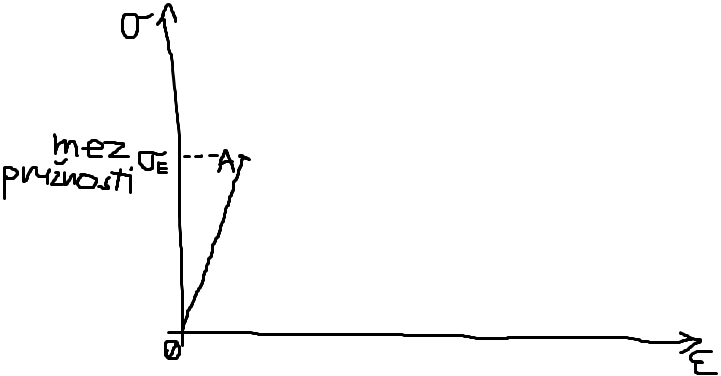
\includegraphics[width=0.75\linewidth]{deformacni_krivka}\vspace{-0.25cm}
      \end{center}

      \begin{itemize}
        \item lineární úsek (0 - A)
        \begin{itemize}
          \item pružná deformace
          \item vratná
          \item platí Hookův zákon:
            \begin{equation}
              \varepsilon \propto \sigma
              \end{equation}
          tedy slovy: relativní prodloužení je přímo úměrné napětí (ano, to je symbol pro přímou úměrnost, zapamatujte si ho)
            \begin{equation}
              \sigma = E*\varepsilon
            \end{equation}
          E - Youngův modul pružnosti (např. ocel = 220 GPa, cín = 55 GPa, tj. tlak potřebný, abychom objekt roztáhli na dvojnásobnou délku)
        \end{itemize}
        \item potrolenicko
      \end{itemize}

\end{document}
